%@+leo-ver=4-thin
%@+node:hasletpara.20130905084546.1629:@shadow ./fmpp/Tex/Proposal.tex
%@@language latex
%Version number 1.0
\documentclass[12pt]{CRPITStyle} 
%\usepackage{epsfig} % Packages to use if you wish
%\usepackage{lscape} % 
\usepackage[authoryear]{natbib}
\usepackage{graphicx}
\renewcommand{\cite}{\citep}
\pagestyle{empty}
\thispagestyle{empty}
\hyphenation{roddick}
\onecolumn
\begin{document}

%@<<title>>
%@+node:hasletpara.20130905084546.1630:<<title>>
\title{Thesis Proposal}
\author{Paran D Haslett (300274241)}
\affiliation{School of Engineering and Computer Science\\
Room C168C\\
Cotton Building\\
Victoria University of Wellington\\
Gate 6, Kelburn Parade\\
Wellington, \\
Email :~{\tt Paran.Haslett@ecs.vuw.ac.nz}}
%@nonl
%@-node:hasletpara.20130905084546.1630:<<title>>
%@nl
\maketitle

%@<<abstract>>
%@+node:hasletpara.20130905084546.1631:<<abstract>>
\begin{abstract}
When collaborating on a project there are times when the code diverges. This could be due to refactoring or the code being reused in another project. It could even be due to throw away code or code used for debugging. This could at times also involve how the structure of the program is presented or the variable and method names that are being used. This is especially true if there is a piece of functionality that you wish to work on that differs from what everyone else is working on. In these cases you may need to refactor the code to best suit your changes before you apply them. The ability to have a separate view which although functionally equivalent to other views can present the code in a different form in these situations would be valuable. It enables the programmer to refactor or change the code with minimal impact on others. If the relationships between views are maintained it also could better recognise the changes that need to be communicated to other views or branches.
\end{abstract}
\vspace{.1in}

\noindent {\em Keywords: Personal annotations, Collaboration, Multiple views, Semantic Merge, Refactoring} 
%@nonl
%@-node:hasletpara.20130905084546.1631:<<abstract>>
%@nl

%@<<body>>
%@+node:hasletpara.20130905084546.1632:<<body>>
%@+others
%@+node:hasletpara.20130905084546.1650:Introduction
\section{Introduction}
There are some issues that arise in Software Development when code diverges from a point. This divergence could be caused for a number of reasons including adding new functionality, refactoring, or code being reused. When source code diverges it could be helpful to retain relationships between the two distinct branches or views. In keeping these relationships it may be useful to identify source code that has the same functionality or source code that is only relevant within a particular branch or view. 

%@+others
%@+node:hasletpara.20130905084546.1662:The problem
%@+others
%@+node:hasletpara.20130905084546.1667:refactoring
\subsection{Refactoring}
A common concern with coding is the need to periodically refactor the code. According to Fowler et al. the main time for refactoring is when new functionality is added \cite{Fowler1999}. Similarly according to Kerievsky some of the motivations for refactoring include adding more code and understanding existing code \cite{Kerievsky2004}. As adding more functionality is one of the motivations for refactoring let us consider what happens in a multi-developer environment. Two developers could have different views on what is considered an appropriate refactoring. This is especially true if they need to add different functionality from each other. 

A simple example is illustrated as follows:
\begin{verbatim}
public TempConv() {
  %@  <<tempConv>>
  %@+node:hasletpara.20131120092329.1771:<<tempConv>>
  Scanner keyboard = new Scanner(System.in);
  System.out.println("Enter the temperature in Celsius");
  int celsius = keyboard.nextInt();
  System.out.println("Degrees Fahrenheit is approx " + (celsius * 2 + 30) );
  keyboard.close();
  %@nonl
  %@-node:hasletpara.20131120092329.1771:<<tempConv>>
  %@nl
}
\end{verbatim}

Refactoring this code depends on what functionality you need to add. One developer may recognize that conversion from Celsius may be used several times throughout the code and so extract the calculations as a separate method as follows:

\begin{verbatim}
public TempConv() {
  %@  <<tempConv2>>
  %@+node:hasletpara.20131120092329.1772:<<tempConv2>>
  Scanner keyboard = new Scanner(System.in);
  System.out.println("Enter the temperature in Celsius");
  int celsius = keyboard.nextInt();
  System.out.println("Degrees Fahrenheit is approx " + celsiusToFahrenheit(celsius));
  keyboard.close();
  %@nonl
  %@-node:hasletpara.20131120092329.1772:<<tempConv2>>
  %@nl
}

public int celsiusToFahrenheit(int celsius){
  %@  <<celsiusToFahrenheit>>
  %@+node:hasletpara.20131120092329.1773:<<celsiusToFahrenheit>>
  return celsius * 2 + 30;
  %@nonl
  %@-node:hasletpara.20131120092329.1773:<<celsiusToFahrenheit>>
  %@nl
}
\end{verbatim}

This change, in spite of producing the same output as the first, provides a number of advantages. Firstly if other programs need to convert from Celsius to Fahrenheit the new method can easily be reused. Secondly since the calculation is a crude estimation it becomes a lot clearer where the code needs to be changed to improve the formula. The ability to add a method that clearly indicates that the calculation is from Celsius to Fahrenheit helps with the readability of the code. There are also disadvantages to doing this refactoring however. If we do not care about conversion between Celsius and Fahrenheit the refactoring simply adds to the amount of code we need to wade through before understanding what the code does. An alternate way of refactoring is as follows:

\begin{verbatim}
public TempConv(){
  %@  <<tempConv3>>
  %@+node:hasletpara.20131120092329.1774:<<tempConv3>>
  Scanner keyboard = new Scanner(System.in);
  System.out.println("Enter the temperature in Celsius");
  int celsius = keyboard.nextInt();
  int celsiusToFahrenheit = celsius *2 + 30;
  System.out.println("Degrees Fahrenheit is approx " + celsiusToFahrenheit);
  keyboard.close();
  %@nonl
  %@-node:hasletpara.20131120092329.1774:<<tempConv3>>
  %@nl
}
\end{verbatim}

While this again expresses the same functionality as the code above it has not created a new method to do so. This has some of the same advantages. It separates and identifies the formula to convert between Celsius and Fahrenheit. It also uses less code to express this separation than forming a new method. It does not expose the conversion formula outside this method to be used by other calculations however.

As the value of a particular refactoring appears to depend on what is trying to be achieved it is very hard to claim that one refactoring is better than another. It depends entirely on the wider context of the intention for the refactoring, in this case the level of access required for the approximation to convert Celsius to Fahrenheit.

Although this was a simple example it is easy to imagine a case where a much larger refactoring process is undertaken. In such circumstances a merge becomes difficult. 
%@-node:hasletpara.20130905084546.1667:refactoring
%@+node:hasletpara.20130905084546.1664:Differences in understanding code
\subsection{Differences in how code is understood}
Another reason that Kerievsky claims for refactoring code is to better understand it \cite{Kerievsky2004}. The very act of going through the source code and reprocessing it in a clearer form can help with the understanding of it. This would suggest that developers tend to leave the code in a difficult to understand state or that different developers understand things differently.
Kerievsky also relates a tale about how the lack of knowledge of patterns making a particular refactoring look a lot more complex \cite{Kerievsky2004}. The different perspectives meant that the programmer he refers to as John has a differing opinion that the refactored code was not an improvement. This shows that it is not just different functionality that influences the need to refactor but sometime the knowledge and experience of the developers themselves. It is often the case that two developers could have different views about what is an appropriate refactoring. This could be because each person brings different skills, notices different issues and has a preferred way of visualizing a problem and solution.

%@-node:hasletpara.20130905084546.1664:Differences in understanding code
%@+node:hasletpara.20131104103532.1627:Multiple developers
\subsection{Working on large projects with multiple developers}
Perry claimed that there are not adequate tools to use with projects with multiple developers \cite{Perry2001}. Whilst a lot of differences between two different versions of source code can be already merged by source control, refactoring often involves larger structural changes. According to Freese these larger changes can lead to merge problems if a traditional text difference approach is used \cite{freese2007operation}. Digg et al. have identified that merging after refactoring causes problems with some SCM systems and tools that are more aware of semantic changes are necessary \cite{Dig2008}. This has lead to the development of smarter merge technology being used to compare code. The simplest of these being hunting for regular expressions so that white-space is not a factor during merging. This is already a feature on many merge tools. Some more complicated examples of these are presented by Le{\ss}enich and Apel who both identify in addition to text based merging both structured and semi-structured approaches to merging \cite{LeBenich2012} \cite{Apel2011}. Although Le{\ss}enich briefly talks about using GIT with a semi structured merge they have named ``JDime'' there are some interesting features of a distributed version control system that have not been explored.

\begin{center}
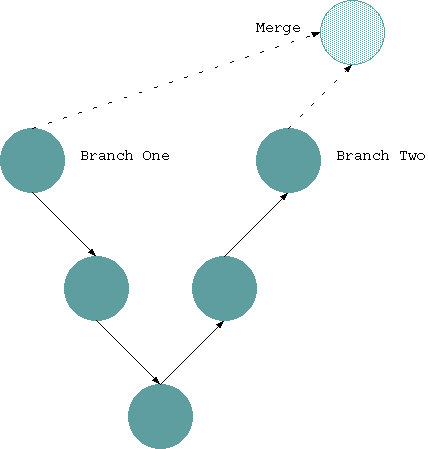
\includegraphics[scale=0.5]{git-diag}
\end{center}

In the above diagram we have a situation where two branches have diverged in GIT and we would like to merge only the changes that would have a \emph{functional difference}. We do not want to merge differences in branch one if they have been refactored but still perform the same function as branch two. There has been some success in using JDime to achieve this. JDime can do a refactoring based merge on the head of branch one with the head of branch two. As a refactoring merge is done from the head of each branch the code may have diverged a great distance. There may be benefits in instead doing a lot of micro refactoring merges, one for each check-in. As the code has not diverged as far for a single check-in, the conflicts could be less severe and easier to automatically resolve. 

Let us also consider if both branches in a merge have been refactored or dramatically changed. During a merge it would be advisable to favour one set of changes over another and then work through the conflicts. While this might be appropriate there could be times when further changes need to be made on the branch with the unfavoured refactoring. This would be true if there were periodic updates of functionality. When the next merge occurs for the diverging branches we could find ourselves having to resolve similar merge conflicts. 

%@-node:hasletpara.20131104103532.1627:Multiple developers
%@-others
%@nonl
%@-node:hasletpara.20130905084546.1662:The problem
%@-others
%@-node:hasletpara.20130905084546.1650:Introduction
%@+node:hasletpara.20130905084546.1653:Related Work
\section{Related Work}
The ability to have two different refactored views of a functionally equivalent piece of source code is influenced by a number of software practices and tools. Some of these allow different views to interact by requiring them to adhere to certain standards and some are more flexible. The challenge is to allow flexibility while communicating what a change in one view should mean to the other. 

%@+others
%@+node:hasletpara.20130910094414.1578:Archetecture
\subsection{Formal architecture and design}
An approach that has been tried in an effort to manage different points of view is by ensuring that the source code has a strictly agreed upon architecture. The architecture could change dramatically when refactoring in order to add further functionality. According to Tang et al. a reason you might want to change an architecture is that is often hard to determine an appropriate design before something is implemented \cite{Tang2009}. A dramatic change to the architecture could mean a greater number of people who are affected by that change. The people who are affected may have to revise their understanding of the new structure even if it still performs the same function as before. It also requires the intervention of an architect and assumes that there is if not one right way to represent code that should be chosen and agreed upon. Taylor et al. claims that there will always be the need for design \cite{Taylor2007}. What this view overlooks however is that a different perspective or different design may be better suited to a different task. Even Taylor et al.spends quite some time discussing different perspectives and paradigms but does not develop this further into an understanding that there could be equivalently well designed artefacts for the same purpose that differ \cite{Taylor2007}.
%@nonl
%@-node:hasletpara.20130910094414.1578:Archetecture
%@+node:hasletpara.20131031084746.1626:Big ball of mud
\subsection{Big Ball of Mud}
According to Foote throwaway code is a major cause for the most often coded Big Ball of Mud pattern \cite{Foote1997}. Some of this could be made worse by source control merges not being able to identify the throwaway code. In practice these are normally marked with a comment to manually indicate that this code is irrelevant or temporary and needs revision. The source control system is not aware about these comments and does not identify the throwaway code. Quick and dirty fixes can make their way from the branches into the main stream without being checked to see if they are wanted.
%@nonl
%@-node:hasletpara.20131031084746.1626:Big ball of mud
%@+node:hasletpara.20131115102112.1758:Code equivlency
\subsection{Code Equivalence}
The ability to detect code that has the same functionality is especially relevant to this thesis. Park et al. have suggested one way that this could be achieved however this may be too coarse grained \cite{Park2013}. Park suggests using some very basic rules to eliminate items in the compared source code that have very little impact on how the program functions. An example would be changing all string arguments ("string") into empty strings ("") before comparing the code. This requires ignoring items that could be relevant later. Using Parks method still may be a good initial step to determine if code blocks underwent large structural changes. The semi-semantic merge suggested by Le{\ss}nich and Apel may be a better approach \cite{LeBenich2012} \cite{Apel2011}.
%@nonl
%@-node:hasletpara.20131115102112.1758:Code equivlency
%@+node:hasletpara.20130910094414.1579:Design patterns
\subsection{Design patterns}
Design patterns are another way which has been used to identify the best code for a particular issue. Due to the dynamic nature of source code however it may be useful to consider different design patterns for differing tasks. Designing according to patterns without making a clear judgement call about if the pattern is necessary could lead to a condition Kerievsky calls ``Patterns Happy'' \cite{Kerievsky2004}. This refers to code as being over-engineered. This means there could still be some dispute about the correct pattern to use in a certain situation. Therefore it is possible for code to diverge even if patterns are used.
%@nonl
%@-node:hasletpara.20130910094414.1579:Design patterns
%@+node:hasletpara.20130910094414.1581:Model Driven Development
%@-node:hasletpara.20130910094414.1581:Model Driven Development
%@+node:hasletpara.20130910094414.1583:Mviews
\subsection{MViews}
MViews as described by Grundy is a way to have multiple different views of the code\cite{Grundy1993}. This is of interest to us because we want to be able to maintain two different refactored versions of the code. The way that this thesis differs from the work done by Grundy is instead of using a centralised database to store common information we are interested in maintaining two self-contained views.
%@nonl
%@-node:hasletpara.20130910094414.1583:Mviews
%@+node:hasletpara.20131105141303.1629:reuse
\subsection{Reuse}
Another reason you may want to diverge from a point is when the code is being reused. Tracz claims that often it needs to be refactored to fit in with the new code \cite{Tracz1995}. Once it has been refactored any further changes in the original code need to be manually propagated. Normally this is how you would expect a typical reuse scenario if the code can be used without the refactoring. If we consider one form of reuse being the use of library packages however sometimes when the library package updates the programmer may want to use the new library. Having the ability to make updating a smaller block of code smoother in spite of it being refactored may be desirable. 
%@nonl
%@-node:hasletpara.20131105141303.1629:reuse
%@+node:hasletpara.20130910094414.1582:version control
\subsection{Version Control} 
A way to maintain divergent code that is currently being used is version control. According to Bertino it is possible to keep a smaller more easily deployed repository by evaluating what is necessary and what is unnecessary \cite{Bertino2012}. Although Bertino refers to unnecessary files this premise may also be applicable for the smaller blocks of code we are interested in. This suggests that maintaining a record about what is relevant and what is irrelevant may have some benefit. Version control still can have merge conflict issues. These issues have a far greater chance of occurring if there is a dramatic change such as refactoring. By using a semi-semantic merge as proposed by Apel these issues can be reduced \cite{Apel2011}. The idea of a refactoring aware version control is not new as Freese also proposed a prototype eclipse plug-in for making the version control aware about refactoring code \cite{Freese2006}. What this paper will investigate is if by maintaining information about equivalent relationships and by examining the changes between subsequent check-in if merge conflicts are further reduced. 
%@-node:hasletpara.20130910094414.1582:version control
%@+node:hasletpara.20130910094414.1580:Well Documented Code
%@-node:hasletpara.20130910094414.1580:Well Documented Code
%@-others
%@nonl
%@-node:hasletpara.20130905084546.1653:Related Work
%@+node:hasletpara.20130905084546.1652:Proposed Approach
\section{Proposed Approach}
The ability to represent similar functionality in two different ways could allow developers to refactor for different purposes. However when creating different views or branches merging becomes difficult. By making use of the functional relationships that already exist in JDime and GIT we hope to reduce merge conflicts. 

%@<<Implemenatation>>
%@+node:hasletpara.20131122093500.1838:<<Implemenatation>>
\subsection{Implementation}

The intention of this thesis is to make merging between two diverging branches simpler in three ways. 

\begin{enumerate}

 \item by keeping track of blocks of code that are only relevant to one branch or view.
 \item by keeping track of blocks of code that are functionally equivalent between different branches and views.
 \item by merging the refactoring aware changes in JDime with GIT

\end{enumerate}

There are a number of small blocks of code which may be of importance to only one view.  An example is code that is used solely for debugging. If these can be marked as not needing to be merged it could prevent some merge conflicts. There are a couple of ways in which we may be able to deal with these blocks of code.

The first way is to allow the programmer to use annotations in the source code. This would indicate to the source control system that the code is not relevant to other views and should not be merged.

The second way is to have two branches to represent all the information necessary for an independent view of the source code.  The first branch would contain only the source code which you are willing to share. The second branch would contain, in addition to this, all the blocks of source code which are private.  According to Chacon at the moment the staging area in GIT uses the staging area to allow files to be marked as ready to merge or not \cite{Chacon2009}. This however is on a file basis rather than based on segments of source code.

Annotations could also be used to indicate code that is functionally the same but refactored differently. We will investigate using an annotation consisting of a unique key between each functionally equivalent item. Having two branches, as mentioned above, may provide us with some less obtrusive options but this will need to be investigated.

There is already some refactoring aware merge tools that have been researched. An example would be the ''JDime'' system proposed by Apel \cite{Apel2011}. Most of these however, are general purpose and have been created as difference or merge tools that can be plugged into various version control systems. What this could mean is that a refactoring aware merge is only done on the head.

\begin{center}
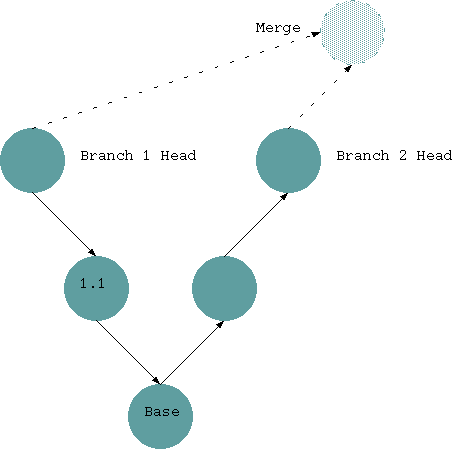
\includegraphics[scale=0.5]{git-diag2}
\end{center}

By combining the functionality of JDime with GIT we aim to use a refactoring based merge between subsequent submissions. Instead of the refactoring aware merge happening between 'Branch 1 Head' and 'Branch 2 Head' we will investigate refactoring aware merges between each of the neighbouring nodes. An example would be doing a refactoring aware merge between 'Base' and '1.1'. As the changes are smaller we expect decreased conflicts when merging. This however means that we will do multiple refactoring-aware merges before getting a result.
%@nonl
%@-node:hasletpara.20131122093500.1838:<<Implemenatation>>
%@nl

%@<<Testing>>
%@+node:hasletpara.20131122093500.1837:<<Testing>>
\subsection{Testing}

For each of the intended changes the number of conflicts will be tested. The dataset we intend to use is the same one as used by Apel et al. so that we can compare how efficient the solution is with JDime on its own \cite{Apel2011}. Some of the conflicts will also be manually examined to see if they are simpler or more simply resolved using the intended changes. 

Because we will often be doing multiple smaller refactoring based merges timing is also going to be an issue. With this in mind we will also be timing the intended changes both independently and together. These will be compared with timings from JDime and text based merges.
%@nonl
%@-node:hasletpara.20131122093500.1837:<<Testing>>
%@nl
%@-node:hasletpara.20130905084546.1652:Proposed Approach
%@-others
%@-node:hasletpara.20130905084546.1632:<<body>>
%@nl

%@<<bibliography>>
%@+node:hasletpara.20130905084546.1649:<<bibliography>>
\bibliography{Thesis}
\bibliographystyle{agsm}
%@nonl
%@-node:hasletpara.20130905084546.1649:<<bibliography>>
%@nl
\end{document}
%@-node:hasletpara.20130905084546.1629:@shadow ./fmpp/Tex/Proposal.tex
%@-leo
